\chapterimage{orange2.jpg} % Chapter heading image
\chapterspaceabove{6.75cm} % Whitespace from the top of the page to the chapter title on chapter pages
\chapterspacebelow{7.25cm} % Amount of vertical whitespace from the top margin to the start of the text on chapter pages

\chapter{Lyapunov Stability I: Autonomous Systems}\index{Introduction}

\section{Overview}\index{Overview}
In this chapter, we introduce the concept of Lyapunov stability for autonomous systems. The main objective is to analyze the qualitative behavior of dynamical systems without explicitly solving the differential equations. Lyapunov’s direct method provides a systematic way to assess the stability of equilibrium points by constructing an energy-like function, called a Lyapunov function. 
This approach is particularly powerful because it applies to nonlinear systems where exact solutions are often difficult or impossible to obtain. We also discuss different notions of stability such as stability in the sense of Lyapunov, asymptotic stability, and global stability, laying the foundation for further analysis of nonlinear control systems.

\section{Basic Definitions}\index{Basic Definitions}

Consider the autonomous system
\begin{equation}
    \dot{x} = f(x), \quad x \in \mathbb{R}^n,
\end{equation}
with an equilibrium point $x_e$ such that $f(x_e) = 0$.

\begin{definition}[Stability]
The equilibrium point $x_e$ is said to be \textbf{stable in the sense of Lyapunov} if for every $\varepsilon > 0$, there exists a $\delta > 0$ such that
\[
    \|x(0) - x_e\| < \delta \quad \Rightarrow \quad \|x(t) - x_e\| < \varepsilon, \ \forall t \geq 0.
\]
\end{definition}

\begin{definition}[Convergence]
The equilibrium point $x_e$ is said to be \textbf{convergent} if
\[
    \lim_{t \to \infty} \|x(t) - x_e\| = 0.
\]
\end{definition}

\begin{definition}[Asymptotic Stability]
The equilibrium point $x_e$ is said to be \textbf{asymptotically stable} if it is both stable (in the sense of Lyapunov) and convergent. That is,
\[
    \|x(0) - x_e\| < \delta \quad \Rightarrow \quad 
    \lim_{t \to \infty} \|x(t) - x_e\| = 0.
\]
\end{definition}

\begin{definition}[Exponential Stability]
The equilibrium point $x_e$ is said to be \textbf{exponentially stable} if there exist constants $c > 0$, $\alpha > 0$, and $\delta > 0$ such that
\[
    \|x(0) - x_e\| < \delta \quad \Rightarrow \quad 
    \|x(t) - x_e\| \leq c \, e^{-\alpha t} \, \|x(0) - x_e\|, \quad \forall t \geq 0.
\]
\end{definition}

%---------------------------------------
\section{Geometric Illustration of Stability}

\begin{figure}[h!]
    \centering
    
    % Circle radii (consistent across all subfigures)
    \def\epsrad{1.5}
    \def\deltarad{0.7}
    
    %---------------- (a) Stability ----------------
    \begin{subfigure}[b]{0.45\textwidth}
    \centering
    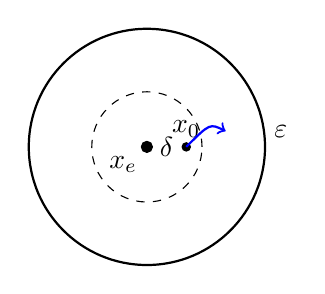
\begin{tikzpicture}[scale=1.0]
        % epsilon circle
        \draw[thick] (0,0) circle (\epsrad);
        \node at (\epsrad+0.2,0.2) {$\varepsilon$};
        % delta circle
        \draw[dashed] (0,0) circle (\deltarad);
        \node at (0.25,0.0) {$\delta$};
        % equilibrium
        \filldraw[black] (0,0) circle (2pt) node[below left] {$x_e$};
        % initial point x0
        \filldraw[black] (0.5,0.0) circle (1.5pt) node[above] {$x_0$};
        % trajectory: stays within epsilon
        \draw[->,blue,thick] (0.5,0.0) .. controls (0.8,0.3) .. (1.0,0.2);
    \end{tikzpicture}
    \caption{Stable: perturbation remains inside $\varepsilon$}
    \end{subfigure}
    \hfill
    %---------------- (b) Convergent ----------------
    \begin{subfigure}[b]{0.45\textwidth}
    \centering
    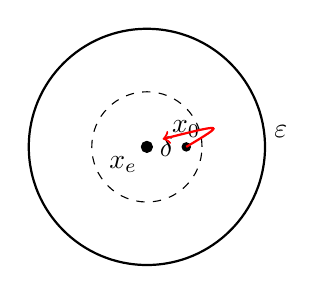
\begin{tikzpicture}[scale=1.0]
        % epsilon circle
        \draw[thick] (0,0) circle (\epsrad);
        \node at (\epsrad+0.2,0.2) {$\varepsilon$};
        % delta circle
        \draw[dashed] (0,0) circle (\deltarad);
        \node at (0.25,0.0) {$\delta$};
        % equilibrium
        \filldraw[black] (0,0) circle (2pt) node[below left] {$x_e$};
        % initial point x0
        \filldraw[black] (0.5,0.0) circle (1.5pt) node[above] {$x_0$};
        % trajectory: moves outward then comes back
        \draw[->,red,thick] (0.5,0.0) .. controls (1.0,0.3) .. (0.2,0.1);
    \end{tikzpicture}
    \caption{Convergent: trajectories return to $x_e$}
    \end{subfigure}
    
    \vspace{0.8cm}
    
    %---------------- (c) Asymptotic stability ----------------
    \begin{subfigure}[b]{0.45\textwidth}
    \centering
    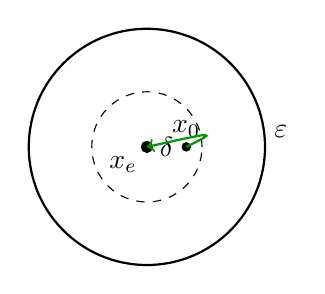
\begin{tikzpicture}[scale=1.0]
        % epsilon circle
        \draw[thick] (0,0) circle (\epsrad);
        \node at (\epsrad+0.2,0.2) {$\varepsilon$};
        % delta circle
        \draw[dashed] (0,0) circle (\deltarad);
        \node at (0.25,0.0) {$\delta$};
        % equilibrium
        \filldraw[black] (0,0) circle (2pt) node[below left] {$x_e$};
        % initial point x0
        \filldraw[black] (0.5,0.0) circle (1.5pt) node[above] {$x_0$};
        % trajectory: goes slightly outward then converges back
        \draw[->,green!60!black,thick] (0.5,0.0) .. controls (0.9,0.2) .. (0.0,0.0);
    \end{tikzpicture}
    \caption{Asymptotically Stable: stable + convergent}
    \end{subfigure}
    \hfill
    %---------------- (d) Exponential stability ----------------
    \begin{subfigure}[b]{0.45\textwidth}
    \centering
    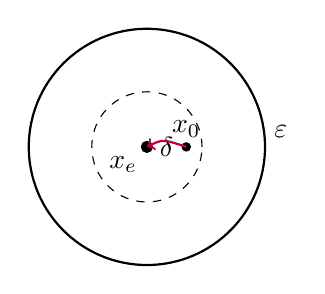
\begin{tikzpicture}[scale=1.0]
        % epsilon circle
        \draw[thick] (0,0) circle (\epsrad);
        \node at (\epsrad+0.2,0.2) {$\varepsilon$};
        % delta circle
        \draw[dashed] (0,0) circle (\deltarad);
        \node at (0.25,0.0) {$\delta$};
        % equilibrium
        \filldraw[black] (0,0) circle (2pt) node[below left] {$x_e$};
        % initial point x0
        \filldraw[black] (0.5,0.0) circle (1.5pt) node[above] {$x_0$};
        % trajectory: sharp fast decay to equilibrium
        \draw[->,purple,thick] (0.5,0.0) .. controls (0.2,0.1) .. (0.0,0.0);
    \end{tikzpicture}
    \caption{Exponentially Stable: fast decay $\sim e^{-\alpha t}$}
    \end{subfigure}

    \caption{Illustrations of stability concepts around equilibrium $x_e$: 
    all trajectories start at an initial condition $x_0$ inside the $\delta$-ball 
    and evolve differently depending on the stability type.}
\end{figure}

